\documentclass[10pt]{article}
\usepackage[margin=0.62in]{geometry}
\usepackage{amsmath,amssymb,xcolor,tikz,tikz-cd,fancyvrb,fontspec,enumitem,booktabs}
\usetikzlibrary{arrows.meta,calc,fit,positioning,shapes.geometric}
\pagestyle{empty}
\setlength{\parindent}{0pt}
\setlength{\parskip}{3pt}
\setlist{nosep,leftmargin=1.35em}
\definecolor{navy}{RGB}{35,75,130}
\definecolor{good}{RGB}{30,120,82}
\definecolor{warn}{RGB}{166,92,16}
\definecolor{bad}{RGB}{151,42,49}
\definecolor{pale}{RGB}{242,246,250}
\newfontfamily\leanfont{DejaVu Sans}
\newenvironment{lean}{\Verbatim[fontsize=\scriptsize,frame=single,framesep=1.5mm,rulecolor=\color{navy},formatcom=\leanfont]}{\endVerbatim}
\newcommand{\idim}{\operatorname{idim}}
\begin{document}

\begin{center}
{\Large\bfseries Final readiness review: \texttt{InjectiveDimension}}\\[-1mm]
\small Lean 4 practice \;·\; categorical shape \;·\; merge decision
\end{center}

\begin{center}
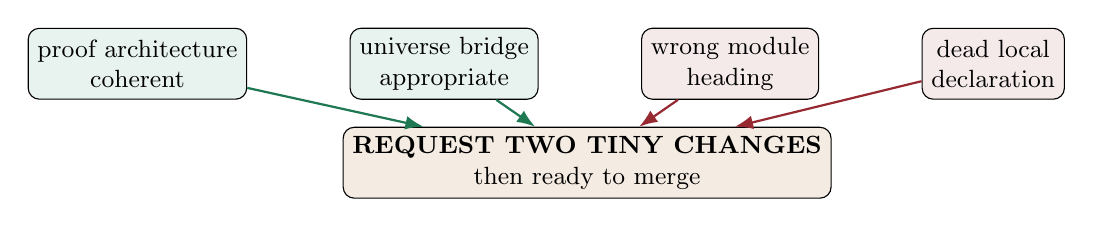
\begin{tikzpicture}[>=Latex,node distance=8mm and 13mm,
 box/.style={draw,rounded corners,align=center,minimum height=9mm,font=\small}]
\node[box,fill=good!10] (math) {proof architecture\\coherent};
\node[box,fill=good!10,right=of math] (uv) {universe bridge\\appropriate};
\node[box,fill=bad!10,right=of uv] (title) {wrong module\\heading};
\node[box,fill=bad!10,right=of title] (dead) {dead local\\declaration};
\node[box,fill=warn!12,below=of $(uv)!0.5!(title)$] (decision) {\textbf{REQUEST TWO TINY CHANGES}\\then ready to merge};
\draw[->,good,thick] (math)--(decision);
\draw[->,good,thick] (uv)--(decision);
\draw[->,bad,thick] (title)--(decision);
\draw[->,bad,thick] (dead)--(decision);
\end{tikzpicture}
\end{center}

\section*{Decision}
\begin{tabular}{@{}p{0.17\linewidth}p{0.76\linewidth}@{}}
\toprule
\textbf{As posted} & \textcolor{bad}{\textbf{Not quite ready}}: two source cleanups should land first.\\
\textbf{After fixes} & \textcolor{good}{\textbf{Ready}} from the proof/API review perspective.\\
\textbf{Validation} & Run the target Mathlib build, linter, and minimum-import check on the PR branch.\\
\bottomrule
\end{tabular}

\section*{Required before merge}
\textbf{1. Correct the file heading.}
\begin{lean}
- # Projective Dimension in ModuleCat
+ # Injective Dimension in ModuleCat
\end{lean}
A one-line scope sentence should mention invariance under linear and ring-semilinear equivalences,
including different universes.

\textbf{2. Delete the unused declaration; use \texttt{exact}.}
\begin{lean}
- have := exactS.hasInjectiveDimensionLT_X₃_iff n inferInstance
- apply (exactS.hasInjectiveDimensionLT_X₃_iff n inferInstance).symm.trans
+ exact (exactS.hasInjectiveDimensionLT_X₃_iff n inferInstance).symm.trans
    ((ih eCoker).trans
      (exactS'.hasInjectiveDimensionLT_X₃_iff n inferInstance))
\end{lean}
The original anonymous \texttt{have} is immediately recomputed and never consumed.  Naming the
quotient equivalence \texttt{eCoker} also avoids overloading \texttt{e}.

\section*{Proof shape: keep}
\begin{center}
\begin{tikzcd}[column sep=1.5em,row sep=2.5em,cells={nodes={font=\small}}]
0 \arrow[r] & M \arrow[r,"f"] \arrow[d,"e_{MN}"',"\sim"]
 & I \arrow[r,"q"] \arrow[d,"e_I"',"\sim"]
 & C=I/\operatorname{range}(f) \arrow[r] \arrow[d,"e_C"',"\sim"] & 0\\
0 \arrow[r] & N \arrow[r,"f'"]
 & I' \arrow[r,"q'"]
 & C'=I'/\operatorname{range}(f') \arrow[r] & 0
\end{tikzcd}
\end{center}
\[
\idim(M)\le n+1
\iff \idim(C)\le n
\iff \idim(C')\le n
\iff \idim(N)\le n+1.
\]
This is the correct induction invariant: injective middle terms, equivalent cokernels, and dimension
shifting.  The base case correctly reduces dimension zero to injectivity and transports it through
Baer's criterion / ring equivalence.

\newpage
\section*{Lean and category-theory review}

\begin{center}
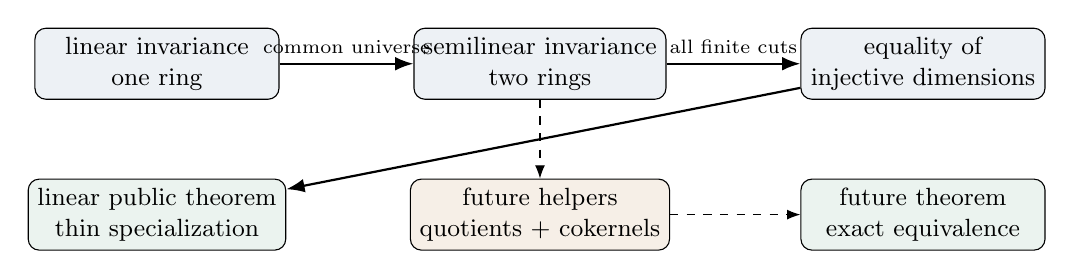
\begin{tikzpicture}[>=Latex,node distance=10mm and 17mm,
 box/.style={draw,rounded corners,align=center,font=\small,minimum width=31mm,minimum height=9mm}]
\node[box,fill=navy!8] (lin) {linear invariance\\one ring};
\node[box,fill=navy!8,right=of lin] (semi) {semilinear invariance\\two rings};
\node[box,fill=navy!8,right=of semi] (dim) {equality of\\injective dimensions};
\draw[->,thick] (lin)--node[above,font=\scriptsize]{common universe}(semi);
\draw[->,thick] (semi)--node[above,font=\scriptsize]{all finite cuts}(dim);
\node[box,fill=good!9,below=of lin] (thin) {linear public theorem\\thin specialization};
\draw[->,thick] (dim)--(thin);
\node[box,fill=warn!10,below=of semi] (helpers) {future helpers\\quotients + cokernels};
\node[box,fill=good!9,below=of dim] (exact) {future theorem\\exact equivalence};
\draw[->,dashed] (semi)--(helpers);
\draw[->,dashed] (helpers)--(exact);
\end{tikzpicture}
\end{center}

\textbf{Good practice to preserve}
\begin{itemize}
\item The public linear result is a one-line specialization of the semilinear theorem.
\item \texttt{ULift} moves both modules explicitly to \(\max(v,v')\); this is clearer than hiding
      the universe transport behind coercions.
\item \texttt{RingHomInvPair.of\_ringEquiv} and the transparency option have narrow lexical scope.
\item The new root import is alphabetically placed after \texttt{Injective}.
\item The theorem states the strongest useful cross-ring, cross-universe result.
\end{itemize}

\textbf{Small source-quality improvements}
\begin{itemize}
\item Put \texttt{hasInjectiveDimensionLE\_iff\_of\_linearEquiv\_aux} in a section that does not
      declare unused \texttt{R'} and outer \texttt{e}; use \texttt{eMN}, \texttt{eI},
      \texttt{eCoker}.
\item Rename the extended-natural cutoff in \texttt{eq\_of\_forall\_ge\_iff} from \texttt{N} to
      \texttt{d}; \texttt{N} already denotes the target module.
\item Name injectivity evidence (for example \texttt{injI'} and \texttt{injI}) rather than relying
      on anonymous local instances when practical.
\end{itemize}
These improve readability but need not expand this PR beyond the two required edits.

\section*{Follow-up API, not a blocker}
\begin{center}
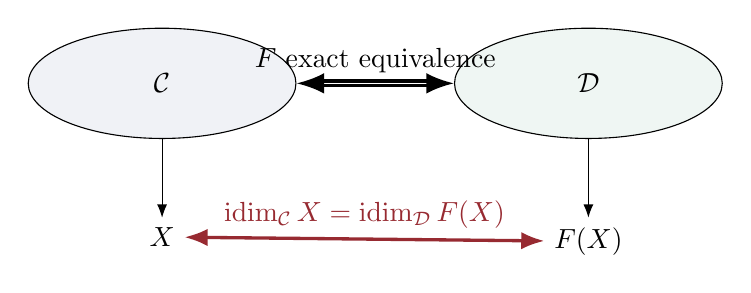
\begin{tikzpicture}[>=Latex,node distance=20mm]
\node[draw,ellipse,fill=navy!7,minimum width=34mm,minimum height=14mm] (C) {$\mathcal C$};
\node[draw,ellipse,fill=good!7,right=of C,minimum width=34mm,minimum height=14mm] (D) {$\mathcal D$};
\draw[<->,double,very thick] (C)--node[above] {$F$ exact equivalence}(D);
\node[below=10mm of C] (x) {$X$};
\node[below=10mm of D] (fx) {$F(X)$};
\draw[->] (C)--(x); \draw[->] (D)--(fx);
\draw[<->,very thick,bad] (x)--node[above] {$\idim_{\mathcal C}X=\idim_{\mathcal D}F(X)$}(fx);
\end{tikzpicture}
\end{center}
Prove injective-dimension invariance once for exact equivalences of abelian categories.  Separately,
add a constructor transporting a semilinear equivalence to quotients when the relevant submodules
map to one another, and package the canonical short exact sequence of an injective linear map.
Those abstractions would remove the low-level \texttt{mapQ}/range bookkeeping from a later refactor.

\section*{Final checklist}
\begin{center}
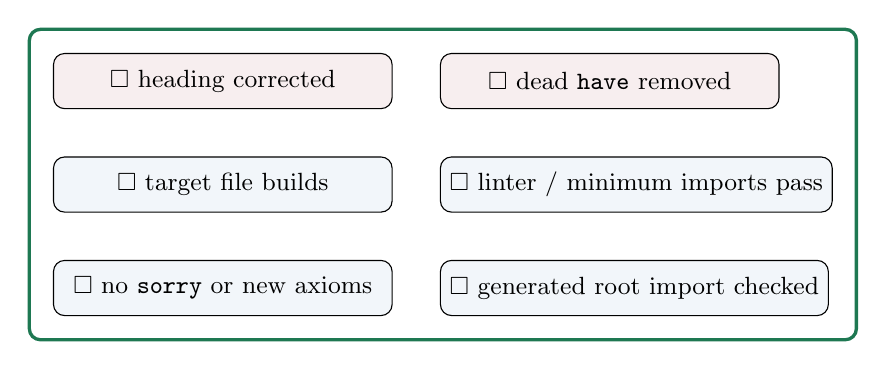
\begin{tikzpicture}[>=Latex,node distance=6mm,
 item/.style={draw,rounded corners,minimum width=43mm,minimum height=7mm,font=\small,align=left}]
\node[item,fill=bad!8] (a) {$\square$ heading corrected};
\node[item,fill=bad!8,right=of a] (b) {$\square$ dead \texttt{have} removed};
\node[item,fill=pale,below=of a] (c) {$\square$ target file builds};
\node[item,fill=pale,right=of c] (d) {$\square$ linter / minimum imports pass};
\node[item,fill=pale,below=of c] (e) {$\square$ no \texttt{sorry} or new axioms};
\node[item,fill=pale,right=of e] (f) {$\square$ generated root import checked};
\node[draw=good,very thick,rounded corners,fit=(a)(b)(c)(d)(e)(f),inner sep=3mm] {};
\end{tikzpicture}
\end{center}

\begin{center}
\colorbox{good!12}{\parbox{0.86\linewidth}{\centering
\textbf{Bottom line:} the mathematics and induction design look mergeable.  Apply the title and
dead-code fixes, verify on the actual PR branch, and approve.}}
\end{center}

\end{document}
